\documentclass[letter]{article}

%\usepackage[letterpaper,right=1.25in,left=1.25in,top=1.25in,bottom=1.25in]{geometry}
\usepackage[longnamesfirst, sort]{natbib}\bibpunct[]{(}{)}{;}{a}{}{,}
\usepackage{ae} % or {zefonts}
\usepackage[T1]{fontenc}
\usepackage[ansinew]{inputenc}
\usepackage{amsmath}
\usepackage{amssymb}
\usepackage{graphicx}
\usepackage{color}
\usepackage[colorlinks]{hyperref}
\usepackage{url}

\usepackage{tikz} % Easier syntax to draw pgf files (invokes pgf automatically)
\usetikzlibrary{arrows,shapes.geometric}

\begin{document}

\title{Drawing a legislature with marbles}
\author{Eric Magar \\ Instituto Tecnol�gico Aut�nomo de M�xico \\ \url{emagar@itam.mx}}
\date{\today}
\maketitle

\begin{center}
  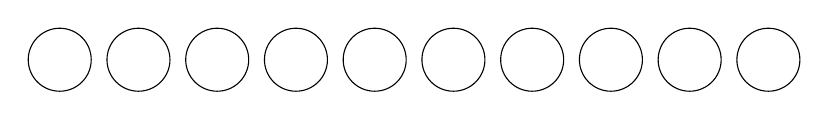
\begin{tikzpicture}[scale=1]
    \foreach \x in {1,...,10}
    \draw (\x,0) circle (.4cm);
  \end{tikzpicture}
\end{center}

\begin{center}
  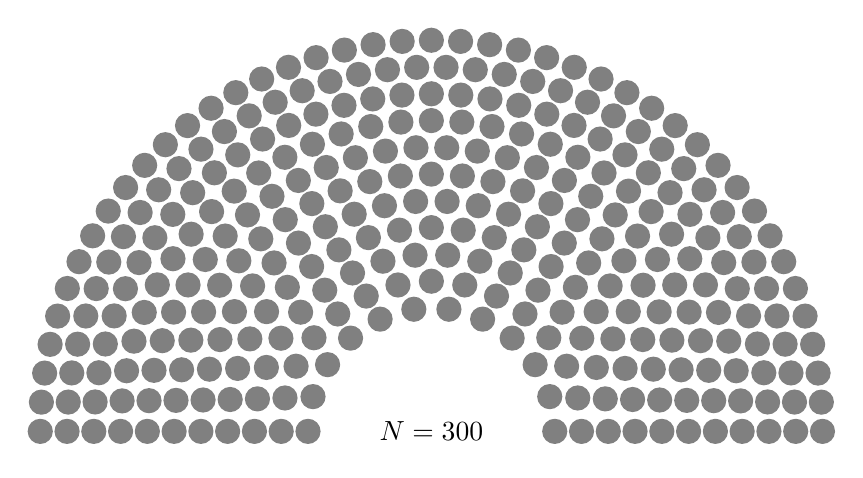
\begin{tikzpicture}[scale=2]
   \def\r{.7835cm} % radius first semi-circle
   \def\b{0.08cm} % ball (marble) radius
   \def\g{0.09cm} % gap between balls (approximate) in between concentric semi-circles
   \def\s{\b+\g} % space between ball centers (approximate) in between concentric semi-circles
   \node (0,0) {$N=300$};
   % row 1 has 11
   \foreach \x in {0,180*1/11,180*2/11,180*3/11,180*4/11,180*5/11,180*6/11,180*7/11,180*8/11,180*9/11,180*10/11,180}
   \fill[black!50] (0,0) + (\x:\r) circle (\b);% node [below=2pt,black] {$x^*$};
   % row 2 has 14
   \def\rtwo{\r+\s} % radius for next concentric circle
   \foreach \x in {0,180*1/14,180*2/14,180*3/14,180*4/14,180*5/14,180*6/14,180*7/14,180*8/14,180*9/14,180*10/14,180*11/14,180*12/14,180*13/14,180}
   \fill[black!50] (0,0) + (\x:\rtwo) circle (\b);% node [below=2pt,black] {$x^*$};
   % row 3 has 17
   \def\rthree{\rtwo+\s} % radius for next concentric circle
   \foreach \x in {0,180*1/17,180*2/17,180*3/17,180*4/17,180*5/17,180*6/17,180*7/17,180*8/17,180*9/17,180*10/17,180*11/17,180*12/17,180*13/17,180*14/17,180*15/17,180*16/17,180}
   \fill[black!50] (0,0) + (\x:\rthree) circle (\b);% node [below=2pt,black] {$x^*$};
   % row 4 has 20
   \def\rfour{\rthree+\s} % radius for next concentric circle
   \foreach \x in {0,180*1/20,180*2/20,180*3/20,180*4/20,180*5/20,180*6/20,180*7/20,180*8/20,180*9/20,180*10/20,180*11/20,180*12/20,180*13/20,180*14/20,180*15/20,180*16/20,180*17/20,180*18/20,180*19/20,180}
   \fill[black!50] (0,0) + (\x:\rfour) circle (\b);% node [below=2pt,black] {$x^*$};
   % row 5 has 23
   \def\rfive{\rfour+\s} % radius for next concentric circle
   \foreach \x in {0,180*1/23,180*2/23,180*3/23,180*4/23,180*5/23,180*6/23,180*7/23,180*8/23,180*9/23,180*10/23,180*11/23,180*12/23,180*13/23,180*14/23,180*15/23,180*16/23,180*17/23,180*18/23,180*19/23,180*20/23,180*21/23,180*22/23,180}
   \fill[black!50] (0,0) + (\x:\rfive) circle (\b);% node [below=2pt,black] {$x^*$};
   % row 6 has 26
   \def\rsix{\rfive+\s} % radius for next concentric circle
   \foreach \x in {0,180*1/26,180*2/26,180*3/26,180*4/26,180*5/26,180*6/26,180*7/26,180*8/26,180*9/26,180*10/26,180*11/26,180*12/26,180*13/26,180*14/26,180*15/26,180*16/26,180*17/26,180*18/26,180*19/26,180*20/26,180*21/26,180*22/26,180*23/26,180*24/26,180*25/26,180}
   \fill[black!50] (0,0) + (\x:\rsix) circle (\b);% node [below=2pt,black] {$x^*$};
   % row 7 has 29
   \def\rseven{\rsix+\s} % radius for next concentric circle
   \foreach \x in {0,180*1/29,180*2/29,180*3/29,180*4/29,180*5/29,180*6/29,180*7/29,180*8/29,180*9/29,180*10/29,180*11/29,180*12/29,180*13/29,180*14/29,180*15/29,180*16/29,180*17/29,180*18/29,180*19/29,180*20/29,180*21/29,180*22/29,180*23/29,180*24/29,180*25/29,180*26/29,180*27/29,180*28/29,180}
   \fill[black!50] (0,0) + (\x:\rseven) circle (\b);% node [below=2pt,black] {$x^*$};
   % row 8 has 32
   \def\reight{\rseven+\s} % radius for next concentric circle
   \foreach \x in {0,180*1/32,180*2/32,180*3/32,180*4/32,180*5/32,180*6/32,180*7/32,180*8/32,180*9/32,180*10/32,180*11/32,180*12/32,180*13/32,180*14/32,180*15/32,180*16/32,180*17/32,180*18/32,180*19/32,180*20/32,180*21/32,180*22/32,180*23/32,180*24/32,180*25/32,180*26/32,180*27/32,180*28/32,180*29/32,180*30/32,180*31/32,180}
   \fill[black!50] (0,0) + (\x:\reight) circle (\b);% node [below=2pt,black] {$x^*$};
   % row 9 has 36
   \def\rnine{\reight+\s} % radius for next concentric circle
   \foreach \x in {0,180*1/36,180*2/36,180*3/36,180*4/36,180*5/36,180*6/36,180*7/36,180*8/36,180*9/36,180*10/36,180*11/36,180*12/36,180*13/36,180*14/36,180*15/36,180*16/36,180*17/36,180*18/36,180*19/36,180*20/36,180*21/36,180*22/36,180*23/36,180*24/36,180*25/36,180*26/36,180*27/36,180*28/36,180*29/36,180*30/36,180*31/36,180*32/36,180*33/36,180*34/36,180*35/36,180}
   \fill[black!50] (0,0) + (\x:\rnine) circle (\b);% node [below=2pt,black] {$x^*$};
   % row 10 has 39
   \def\rten{\rnine+\s} % radius for next concentric circle
   \foreach \x in {0,180*1/39,180*2/39,180*3/39,180*4/39,180*5/39,180*6/39,180*7/39,180*8/39,180*9/39,180*10/39,180*11/39,180*12/39,180*13/39,180*14/39,180*15/39,180*16/39,180*17/39,180*18/39,180*19/39,180*20/39,180*21/39,180*22/39,180*23/39,180*24/39,180*25/39,180*26/39,180*27/39,180*28/39,180*29/39,180*30/39,180*31/39,180*32/39,180*33/39,180*34/39,180*35/39,180*36/39,180*37/39,180*38/39,180}
   \fill[black!50] (0,0) + (\x:\rten) circle (\b);% node [below=2pt,black] {$x^*$};
   % row 11 has 42
   \def\releven{\rten+\s} % radius for next concentric circle
   \foreach \x in {0,180*1/42,180*2/42,180*3/42,180*4/42,180*5/42,180*6/42,180*7/42,180*8/42,180*9/42,180*10/42,180*11/42,180*12/42,180*13/42,180*14/42,180*15/42,180*16/42,180*17/42,180*18/42,180*19/42,180*20/42,180*21/42,180*22/42,180*23/42,180*24/42,180*25/42,180*26/42,180*27/42,180*28/42,180*29/42,180*30/42,180*31/42,180*32/42,180*33/42,180*34/42,180*35/42,180*36/42,180*37/42,180*38/42,180*39/42,180*40/42,180*41/42,180}
   \fill[black!50] (0,0) + (\x:\releven) circle (\b);% node [below=2pt,black] {$x^*$};
 \end{tikzpicture}
\end{center}

Spreadsheet in same directory has template to compute angles and other parameters. Number of legislators can be tweaked. Challenge: color them not by concentric circle, but by column...

\end{document}

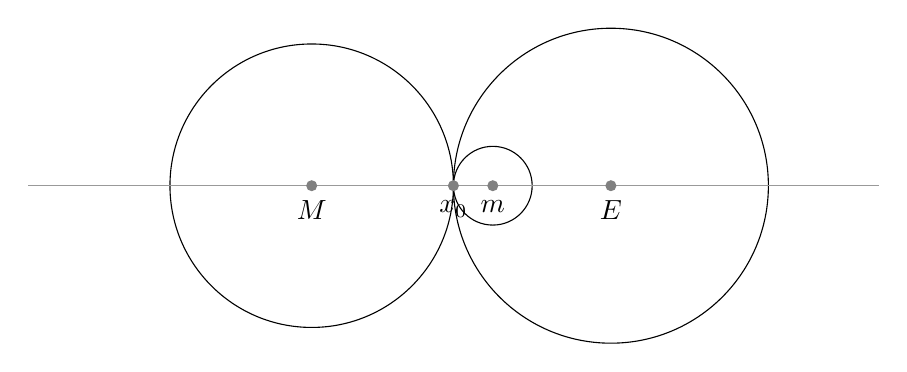
\begin{tikzpicture}[scale=1,rotate=0]
 \def\x0{0,0}
 \def\aE{0} % �ngulo desde el origen (x0)
 \def\lE{2cm} % largo desde el origen
 \def\aM{180}
 \def\lM{1.8cm}
 \def\am{0}
 \def\lm{0.5cm}
% \def\R{1.8cm} % radio del c�rc M tangente con otro winset
% \def\A{20}   % angulo de salida del punto de tangencia
 \def\M{\aM:\lM}
 \def\E{\aE:\lE}
 \def\m{\am:\lm}
 \draw (\M) circle (\lM);
 \draw (\E) circle (\lE);
 \draw (\m) circle (\lm);
% circ M tangente con winset de E
% computes new radius: R = sqrt((\lE*cos(\aE)-\lM*cos(\aM))^2+(\lE*sin(\aE)-\lM*sin(\aM))^2) - \lE
% \draw[dashed] (\M) circle (\R);
%  \begin{scope}
%   \clip (\M) circle (\lM);
%   \fill[black!20] (\E) circle (\lE);
%   \fill[black!20] (\m) circle (\lm);
%  \end{scope}
%  \begin{scope}
%   \clip (\m) circle (\lm);
%   \fill[black!20] (\E) circle (\lE);
%  \end{scope}
%add structure-induced dimension line
 \draw[black!40] (\M)++(\M)++(\M) -- (\x0); %lado izq
 \draw[black!40] ({\aM-180}:\lM)++({\aM-180}:\lM)++({\aM-180}:\lM)--(\x0); %lado der
 \fill[black!50] (\M) circle (2pt) node [below=2pt,black] {$M$};
 \fill[black!50] (\E) circle (2pt) node [below=2pt,black] {$E$};
 \fill[black!50] (\m) circle (2pt) node [below=2pt,black] {$m$};
 \fill[black!50] (\x0) circle (2pt) node [below=2pt,black] {$x_0$};
% \draw (\M) -- (\m) -- (\E) -- (\M); %Pareto set
% adds punto tangente con winset de E
% angle: A = antisin{ \lE*sin(aM-aE) / (R + \lE) } + FALTA compensacion para no arrancar en 0� (ej. si \aM=200: +20�)
% \fill[black!50] (\M) ++(\A:\R) circle (2pt) node [below=2pt,black] {$x^*$};
\end{tikzpicture}



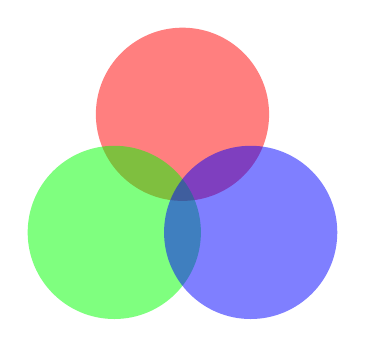
\begin{tikzpicture}
 \pgfsetfillopacity{0.5}
 \fill[red] (90:1cm) circle (11mm);
 \fill[green] (210:1cm) circle (11mm);
 \fill[blue] (-30:1cm) circle (11mm);
\end{tikzpicture}


\begin{tikzpicture}[scale=1,rotate=-12]
 \def\x0{0,0}
 \def\M{180:2}
 \def\E{180:0.6}
 \def\m{0:1.25}
 \draw (-5,0) -- (3,0) node [right=2pt,black] {$X$};
% \draw[black!30] (\M)+(-90:1.25) circle (1.25);
% \draw[black!30] (\E)+(90:.75) circle (.75);
% \draw[black!30] (\m)+(-90:0.75) circle (0.75);
  \begin{scope}
   \clip (-5,0) rectangle (3,2);
    \draw (\M)+(-90:1.25) circle (2.36);
    \draw (\m)+(-90:0.75) circle (1.46);
  \end{scope}
  \begin{scope}
   \clip (-5,0) rectangle (3,-2);
    \draw (\E)+(90:.75) circle (0.96);
  \end{scope}
 \fill[black!50] (\M) circle (1.5pt) node [below=2pt,black] {$M$};
 \fill[black!50] (\E) circle (1.5pt) node [above=2pt,black] {$E$};
 \fill[black!50] (\m) circle (1.5pt) node [below=2pt,black] {$m$};
 \fill[black!50] (\x0) circle (1.5pt) node [below=2pt,black] {$x_0$};
 \fill[black!30] (\M)++(-90:1.2) circle (1.5pt);
 \fill[black!30] (\E)+(90:.75) circle (1.5pt);
 \fill[black!30] (\m)+(-90:.75) circle (1.5pt);
 \fill[black!50] (180:1.2) circle (1.5pt) node [below=2pt,black] {$x^*$};
\end{tikzpicture}


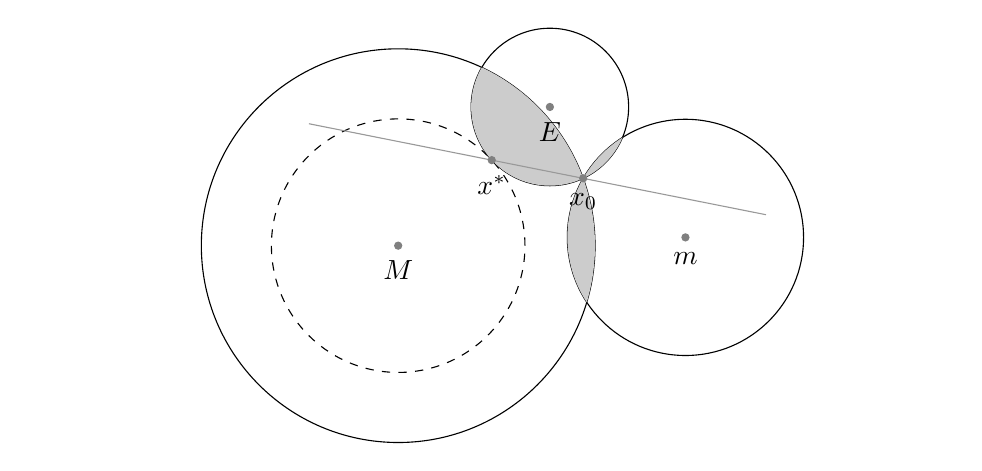
\begin{tikzpicture}[scale=1,rotate=0]
 \def\x0{0,0}
 \def\aE{115} % �ngulo desde el origen (x0)
 \def\lE{1cm} % largo desde el origen
 \def\aM{200}
 \def\lM{2.5cm}
 \def\am{-30}
 \def\lm{1.5cm}
 \def\R{1.61cm} % radio del c�rc M tangente con otro winset
 \def\A{42.43}   % angulo de salida del punto de tangencia
 \def\M{\aM:\lM}
 \def\E{\aE:\lE}
 \def\m{\am:\lm}
 \draw (\M) circle (\lM);
 \draw (\E) circle (\lE);
 \draw (\m) circle (\lm);
% circ M tangente con winset de E
% computes new radius: R = sqrt((\lE*cos(\aE)-\lM*cos(\aM))^2+(\lE*sin(\aE)-\lM*sin(\aM))^2) - \lE
 \draw[dashed] (\M) circle (\R);
  \begin{scope}
   \clip (\M) circle (\lM);
   \fill[black!20] (\E) circle (\lE);
   \fill[black!20] (\m) circle (\lm);
  \end{scope}
  \begin{scope}
   \clip (\m) circle (\lm);
   \fill[black!20] (\E) circle (\lE);
  \end{scope}
%add structure-induced dimension line
 \draw[black!40] (\M)++(\M)++(\M)++(\A:\R)++(\A:\R)++(\A:\R) -- (\x0); %lado izq
 \draw[black!40] ({\aM-180}:\lM)++({\aM-180}:\lM)++({\A-180}:\R)++({\A-180}:\R)--(\x0); %lado der
 \fill[black!50] (\M) circle (1.5pt) node [below=2pt,black] {$M$};
 \fill[black!50] (\E) circle (1.5pt) node [below=2pt,black] {$E$};
 \fill[black!50] (\m) circle (1.5pt) node [below=2pt,black] {$m$};
 \fill[black!50] (\x0) circle (1.5pt) node [below=2pt,black] {$x_0$};
% \draw (\M) -- (\m) -- (\E) -- (\M); %Pareto set
% adds punto tangente con winset de E
% angle: A = antisin{ \lE*sin(aM-aE) / (R + \lE) } + FALTA compensacion para no arrancar en 0� (ej. si \aM=200: +20�)
 \fill[black!50] (\M) ++(\A:\R) circle (1.5pt) node [below=2pt,black] {$x^*$};
\end{tikzpicture}
